\documentclass{standalone}
\usepackage{tikz}
\usepackage{pgfplots}
\begin{document}
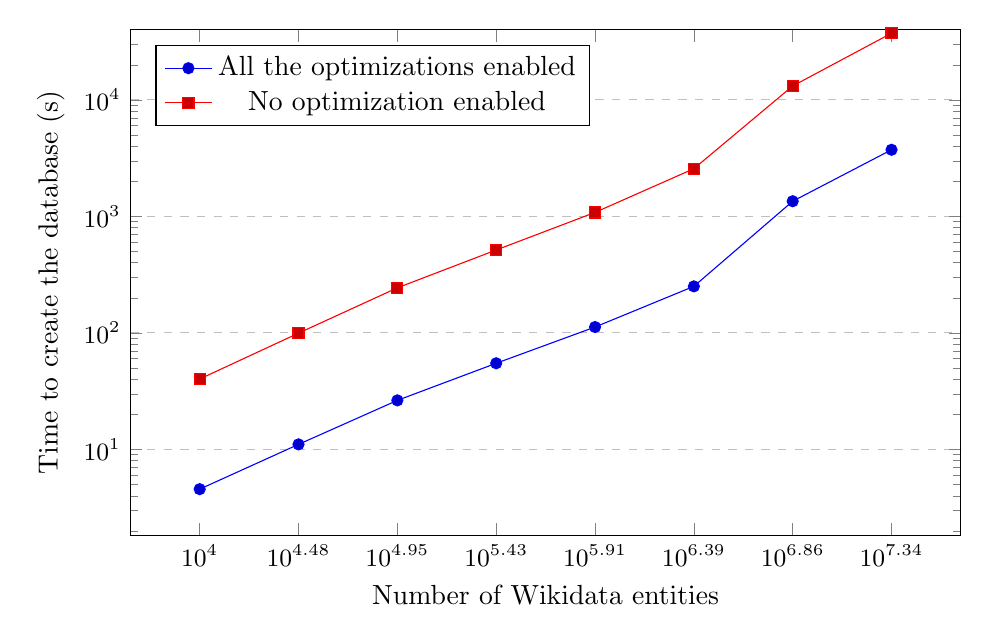
\begin{tikzpicture}
    \begin{axis}[
            title={},
            xlabel={Number of Wikidata entities},
            ylabel={Time to create the database (s)},
            ymin=0, ymax=40000,
            xmode=log,
            ymode=log,
            xtick=data,
            height=8cm,
            width=\textwidth,
            legend pos=north west,
            ymajorgrids=true,
            grid style=dashed,
            tick align=inside,
            every tick label/.append style={font=\small}
        ]
        \addplot coordinates {
                (10000,4.56)
                (30000,11.05)
                (90000,26.36)
                (270000,54.87)
                (810000,112.30)
                (2430000,250.86)
                (7290000,1349.10)
                (21870000,3730.33)
            };
        \addplot coordinates {
                (10000,40.18)
                (30000,99.52)
                (90000,243.64)
                (270000,514.68)
                (810000,1081.64)
                (2430000,2566.25)
                (7290000,13157.18)
                (21870000,37340.60)
            };
        \legend{All the optimizations enabled,No optimization enabled}
    \end{axis}
\end{tikzpicture}
\end{document}